\section{正交展开}
\label{sec:ipspace-orthogonal-expansions}

有了可数的标准正交系，就可以写出级数$\sum_jc_je_j$。第~\ref{chap:functions-as-vectors}章指出，级数要回答三个问题：是否收敛、表示哪些元素、系数是否唯一。本节在Hilbert空间中用范数收敛回答它们：系数由内积给出，有限截断是正交投影，完备正交系给出收敛的展开与能量恒等式，不完备的正交系只恢复它张成的那一部分。

本节设$H$是Hilbert空间，$\{e_j\}$是有限或可数的标准正交系，下标按$j=1,2,\ldots$排列。对$f\in H$，称
\[
 c_j=\langle e_j,f\rangle
\]
为$f$关于$\{e_j\}$的系数。

\paragraph{有限截断是正交投影}
先看只保留有限个方向时的情形。记$M_n=\operatorname{span}\{e_1,\ldots,e_n\}$，它是有限维子空间，因而闭，第~\ref{sec:ipspace-orthogonal-projection}节的结论适用。

\begin{theorem}[有限截断]
\label{thm:ipspace-finite-truncation}
对$f\in H$与$n\geq1$，令$s_n=\sum_{j=1}^nc_je_j$。则$s_n=P_{M_n}f$，并且
\begin{equation}
 \lVert f-s_n\rVert^2=\lVert f\rVert^2-\sum_{j=1}^n\lvert c_j\rvert^2 .
 \label{eq:ipspace-truncation-error}
\end{equation}
\end{theorem}

\begin{proof}
$s_n\in M_n$。对每个$k\leq n$，由标准正交性$\langle e_k,s_n\rangle=\sum_jc_j\langle e_k,e_j\rangle=c_k$，所以$\langle e_k,f-s_n\rangle=c_k-c_k=0$。$f-s_n$与$M_n$的每个基元素正交，因而与$M_n$正交；由正交刻画，$s_n=P_{M_n}f$。再由勾股关系$\lVert f\rVert^2=\lVert s_n\rVert^2+\lVert f-s_n\rVert^2$与$\lVert s_n\rVert^2=\sum_{j\leq n}\lvert c_j\rvert^2$即得式~\eqref{eq:ipspace-truncation-error}。
\end{proof}

这个定理说明，用内积计算的系数就是$M_n$中的最佳选择：在$e_1,\ldots,e_n$的所有组合中，$s_n$离$f$最近。增加一个方向时，已经算好的系数不需要修改，误差平方恰好减少新系数的模平方。若$\{e_j\}$只是线性无关而不正交，这两件事都不成立，系数要重新解一个Gram矩阵方程组。

\paragraph{Bessel不等式}
式~\eqref{eq:ipspace-truncation-error}的左边非负，所以对每个$n$都有$\sum_{j\leq n}\lvert c_j\rvert^2\leq\lVert f\rVert^2$。令$n\to\infty$，得到下面的不等式。

\begin{theorem}[Bessel不等式]
\label{thm:ipspace-bessel}
对$f\in H$，$\sum_j\lvert\langle e_j,f\rangle\rvert^2\leq\lVert f\rVert^2$。
\end{theorem}

非负项级数的部分和有界，所以级数收敛，和不超过这个界。特别地$c_j\to0$：任何元素在越来越靠后的正交方向上的分量都越来越小。这一结论只用到正交系，不要求它完备，也不要求$H$完备。

\paragraph{级数的收敛与和}
Bessel不等式说明系数平方可和。反过来，平方可和的系数总能给出一个收敛的级数，它的和就是$f$在闭张成空间上的投影。

\begin{theorem}[正交展开]
\label{thm:ipspace-orthogonal-expansion}
设$M=\overline{\operatorname{span}}\{e_j\}$。
\begin{enumerate}
 \item 对数列$(a_j)$，级数$\sum_ja_je_j$依范数收敛，当且仅当$\sum_j\lvert a_j\rvert^2<\infty$；此时$\lVert\sum_ja_je_j\rVert^2=\sum_j\lvert a_j\rvert^2$。
 \item 对$f\in H$，级数$\sum_jc_je_j$依范数收敛，其和为$P_Mf$。
\end{enumerate}
\end{theorem}

\begin{proof}
（1）记部分和$t_n=\sum_{j\leq n}a_je_j$。对$n>m$，由标准正交性，$\lVert t_n-t_m\rVert^2=\sum_{m<j\leq n}\lvert a_j\rvert^2$。所以$(t_n)$是柯西列当且仅当$\sum_j\lvert a_j\rvert^2$的部分和是柯西数列，即级数收敛。$H$完备，柯西列收敛；反之收敛列是柯西列。范数等式由$\lVert t_n\rVert^2=\sum_{j\leq n}\lvert a_j\rvert^2$与范数的连续性得到。

（2）由Bessel不等式和（1），$s_n=\sum_{j\leq n}c_je_j$收敛到某个$s$。每个$s_n\in M$，$M$闭，所以$s\in M$。对固定的$k$与$n\geq k$，$\langle e_k,f-s_n\rangle=0$；令$n\to\infty$，由内积的连续性得$\langle e_k,f-s\rangle=0$。于是$f-s$与$\operatorname{span}\{e_j\}$正交，再由连续性与其闭包$M$正交。由正交刻画，$s=P_Mf$。
\end{proof}

（1）中的“仅当”方向不需要完备性，“当”方向需要：在不完备的$c_{00}$中，$\sum_ka_ke_k$对$a_k=1/k$就不收敛。（2）也回答了唯一性：若$\sum_ja_je_j=g$依范数收敛，与$e_k$作内积并取极限，得$a_k=\langle e_k,g\rangle$，系数只能是内积系数。由于（2）对$\{e_j\}$的任何排列都成立，和总是$P_Mf$，所以级数的和不依赖求和次序。

\paragraph{完备正交系：展开与Parseval等式}
若$\{e_j\}$是完备正交系，则$M=H$，$P_Mf=f$，得到最重要的情形。

\begin{theorem}[Parseval等式]
\label{thm:ipspace-parseval}
设$\{e_j\}$是$H$的完备正交系，$f,g\in H$，$c_j=\langle e_j,f\rangle$，$d_j=\langle e_j,g\rangle$。则
\[
 f=\sum_jc_je_j\quad(\text{依范数}),\qquad \lVert f\rVert^2=\sum_j\lvert c_j\rvert^2,\qquad \langle f,g\rangle=\sum_j\overline{c_j}\,d_j .
\]
\end{theorem}

\begin{proof}
展开式由定理~\ref{thm:ipspace-orthogonal-expansion}（2）与$M=H$得到。在式~\eqref{eq:ipspace-truncation-error}中令$n\to\infty$，左边趋于零，得范数等式，称为\term{Parseval等式}（Parseval identity）。对内积，$\langle s_n,t_n\rangle=\sum_{j\leq n}\overline{c_j}d_j$，其中$t_n$是$g$的部分和；由内积的连续性，左边趋于$\langle f,g\rangle$。
\end{proof}

Parseval等式说明，当正交基为可数无穷时，取系数$f\mapsto(c_j)$把$H$一一地映成$\ell^2$，并保持内积：每个$f$给出平方可和的系数，每个平方可和的系数列由定理~\ref{thm:ipspace-orthogonal-expansion}（1）给出唯一的元素。所以一个具有可数正交基的无限维Hilbert空间，在选定正交基后，与$\ell^2$只有记号的差别，就像有限维内积空间选定标准正交基后与$\mathbb K^d$只有记号的差别一样。

由式~\eqref{eq:ipspace-truncation-error}与Parseval等式，截断误差可以直接从系数读出：
\begin{equation}
 \lVert f-s_n\rVert^2=\sum_{j>n}\lvert c_j\rvert^2 ,
 \label{eq:ipspace-tail-error}
\end{equation}
即系数平方的尾和。误差随$n$单调下降并趋于零，下降的快慢完全由系数衰减的快慢决定。

\paragraph{不完备时只恢复闭张成中的部分}
若$\{e_j\}$不完备，展开的和是$P_Mf$而不是$f$，正交补$M^\perp$中的分量永远丢失。Bessel不等式与Parseval等式之间的差$\lVert f\rVert^2-\sum_j\lvert c_j\rvert^2=\lVert f-P_Mf\rVert^2$，正是丢失部分的能量。

回到偶次Legendre多项式。设$E$为$L^2[-1,1]$中几乎处处满足$f(-x)=f(x)$的元素组成的子空间。任意$f$都可以写成$f(x)=\tfrac{f(x)+f(-x)}2+\tfrac{f(x)-f(-x)}2$，前者是偶函数，属于$E$，后者是奇函数，与$E$正交。由正交分解的唯一性，$P_Ef(x)=\tfrac{f(x)+f(-x)}2$，并且$E$就是这个投影的像。偶次Legendre多项式是偶函数，它们的闭张成含于$E$。反过来，对$f\in E$，奇次的$e_k$是奇函数，$\langle e_k,f\rangle=0$；由上一节所述的全体Legendre多项式的完备性，$f$的展开只含偶次项，所以$f$属于偶次Legendre多项式的闭张成。于是这个闭张成恰为$E$，只用偶次方向展开时，和就是$P_Ef$。

取$f=e^x$，得$P_Ef=\cosh x$，丢失的部分是奇部$\sinh x$，见图~\ref{fig:ipspace-even-odd-projection}。距离平方为
\[
 \int_{-1}^1\sinh^2x\,dx=\frac{\sinh2}{2}-1\approx0.813 ,
\]
无论加入多少偶次方向都无法减小。

\begin{figure}[!htb]
  \centering
  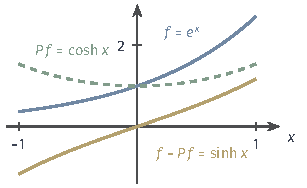
\includegraphics[width=51.9mm]{figures/02-abstract-mathematics/03-function-spaces/tikz/c1-even-odd-projection/figure.pdf}
  \caption{向偶函数子空间的正交投影。$[-1,1]$上$f(x)=e^x$，投影$P_Ef=\cosh x$为其偶部，误差$f-P_Ef=\sinh x$为奇函数，与每个偶函数正交。只用偶次方向展开$e^x$时，误差始终至少为$\lVert\sinh\rVert_2\approx0.90$。}
  \label{fig:ipspace-even-odd-projection}
\end{figure}

\paragraph{截断误差的例子}
用全体Legendre多项式展开符号函数$\operatorname{sgn}$。它是奇函数，只有奇次系数非零，$\lVert\operatorname{sgn}\rVert_2^2=2$。由$e_1=\sqrt{3/2}\,x$，$c_1=\sqrt{3/2}\int_{-1}^1\lvert x\rvert\,dx=\sqrt{3/2}$，$c_1^2=\tfrac32$。由$e_3=\sqrt{7/8}\,(5x^3-3x)$，$\int_{-1}^1\operatorname{sgn}(x)(5x^3-3x)\,dx=2(\tfrac54-\tfrac32)=-\tfrac12$，所以$c_3^2=\tfrac78\cdot\tfrac14=\tfrac7{32}$。同样可算$c_5^2=\tfrac{11}{128}$。由式~\eqref{eq:ipspace-tail-error}，截断误差
\[
 \lVert\operatorname{sgn}-s_1\rVert_2^2=2-\frac32=0.5,\qquad \lVert\operatorname{sgn}-s_5\rVert_2^2=2-\frac32-\frac7{32}-\frac{11}{128}\approx0.195 .
\]

图~\ref{fig:ipspace-legendre-truncation}(a)画出了部分和，(b)把$\operatorname{sgn}$与$\lvert x\rvert$的截断误差放在一起。精确计算给出：$\operatorname{sgn}$在$n=15$时误差约为$0.077$，$n=41$时仍约为$0.030$；$\lvert x\rvert$连续，只在$0$处有折角，$n=2$时误差已约为$0.0104$，$n=40$时约为$6\times10^{-6}$。两者都趋于零，但速度相差很大。这里只是两个例子的观察；系数衰减与函数光滑性之间的一般关系属于第~\ref{chap:function-approximation}章。

\begin{figure}[!htb]
  \centering
  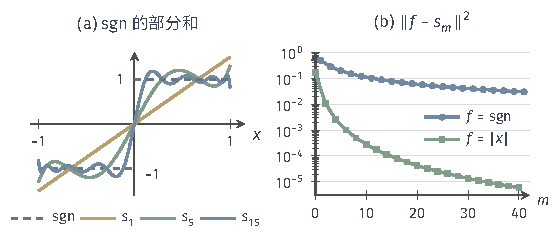
\includegraphics[width=94.9mm]{figures/02-abstract-mathematics/03-function-spaces/tikz/c1-legendre-truncation/figure.pdf}
  \caption{Legendre展开的截断。(a)$\operatorname{sgn}$（虚线）与部分和$s_1,s_5,s_{15}$，其中$s_1=\tfrac32x$；部分和是多项式，在跳跃点附近来回振荡。(b)截断误差$\lVert f-s_n\rVert_2^2$（对数纵轴）：$\operatorname{sgn}$取奇数$n$，$\lvert x\rvert$取偶数$n$。两条曲线都单调趋于零，有跳跃的$\operatorname{sgn}$下降慢得多。}
  \label{fig:ipspace-legendre-truncation}
\end{figure}

\paragraph{范数收敛不是点态收敛}
式~\eqref{eq:ipspace-tail-error}只控制$L^2$误差，不控制任何一点处的值。图~\ref{fig:ipspace-legendre-truncation}(a)中的部分和都是连续函数；若它们一致收敛，极限必然连续，而$\operatorname{sgn}$在$0$处跳跃，没有连续代表，所以部分和不一致收敛到$\operatorname{sgn}$，尽管$L^2$误差趋于零。在$x=0$处，每个部分和都是奇多项式，取值为$0$；而$\operatorname{sgn}$作为$L^2$元素在$0$处根本没有确定的值，谈不上收敛到什么。

更一般地，$L^2$中的元素是等价类，“展开在点$x_0$处收敛到$f(x_0)$”首先要求$f(x_0)$有意义，其次需要“点值受范数控制”这样的额外条件。由第~\ref{chap:normed-spaces}章，$L^2$收敛的序列有几乎处处收敛的子列，但整列部分和是否逐点收敛，要看具体的正交系与函数的正则性。点值读取何时连续，是第~\ref{chap:linear-functionals}章和第~\ref{chap:rkhs}章的问题；三角级数的逐点与一致收敛条件，在第~\ref{chap:fourier-transform}章讨论。
